%!TEX program = <xelatex>
\documentclass[11pt,a4paper]{article}%titlepage表示标题单独页
\usepackage{ctex}%ctex套用英文标题格式(建议在英文论文混排中文时使用),ctexcap套用中文格式(等同于\documentclass{ctexart})
\renewcommand{\figurename}{图}
\renewcommand{\tablename}{表}
%\renewcommand{\thefigure}{\chinese{figure}}%将图片计数改为汉字数字
%\renewcommand{\thetable}{\chinese{table}}%将表格计数改为汉字数字
\usepackage[top=1in,bottom=1in,left=1in,right=1in]{geometry}%页边距设置
\usepackage[CJKbookmarks]{hyperref}%给pdf文档添加互动式链接和书签

\usepackage{amsmath,amssymb,esint}%数学公式类宏包;最末为积分符号拓展
\allowdisplaybreaks[0]%允许多行公式间换页,用//*表示不允许换页
\usepackage{bm}%加粗(用于vector)
%\usepackage{textcomp}%符号包,不能用于数学模式,建议不要和SIunits混用
\usepackage[squaren]{SIunits}%科学单位包,可以用于数学模式(为了统一不要和textcomp混用),squaren选项消除和amssymb的冲突
\usepackage{graphicx}%插图宏包
\usepackage{picinpar}%图文绕排
\usepackage{array}%表格宏包
\usepackage{longtable}%长表格宏包
\usepackage{multirow}%多行合并的表格宏包
%\usepackage{booktabs}%表格线宏包

\usepackage{listings}
\lstset{numbers=left,tabsize=4, xleftmargin=2em,xrightmargin=2em, aboveskip=1em, escapeinside=' '}
\renewcommand{\lstlistingname}{算法}

%\usepackage[basic,box,gate,oldgate,ic,optics,physics]{circ}%电路图宏包
%\usepackage[normalem]{ulem}%下划线,删除线等宏包,参数表示不修改\emph{}格式
%\usepackage{mychemistry}%化学宏包,包含mhchem和chemfig
%\usepackage[symbol]{footmisc}%脚注拓展,选项表示用符号做脚注记号

%\renewcommand*{\vec}[1]{\bm{#1}}%矢量的格式,这里是加粗
\DeclareMathOperator{\dif}{d}
\DeclareMathOperator{\diff}{\, d}
\DeclareMathOperator{\mi}{i}
\DeclareMathOperator{\e}{e}%定义数学模式中常用的正体字符
\renewcommand{\[}{~$}
\renewcommand{\]}{$~}%$只是用来少打空格……
\newcommand{\rank}{\mathrm{rank}\,}

\begin{document}
\title{离散数学-图论整理}
\author{吕铭}
\date{}
\maketitle
\section{基本概念}
	\begin{enumerate}
	 \item 图(Graph)\[G = (V(G), E(G))\]\\
	 	其中\[V(G)\neq \emptyset\]是结点 (vertex) 集,\[E(G)\subseteq V(G)\times V(G)\]是边 (edge) 集
	 	\begin{itemize}
	 	  \item 有向图 (directed graph), 无向图 (undirected graph), 混合图 (mixed graph)
		  \item 自环: 只与一个结点关联的边
		  \item 重边: 若一对结点之间有多条边
		  \item 多重图: 含有重边的图
		  \item 孤立点: 没有关联变的结点
		  \item 简单图: 无重边, 无自环的无向图 
	 	\end{itemize}
	 \item 图的阶 (order)\[|V|=n\](\[n\]阶图),\[|E|=m\]
	 	\begin{itemize}
	 	 \item 完全图\[K_n\]: \[E(K_n) = V(K_n)\times V(K_n)\]
	 	 \item 空图\[N_n\] (null graph / empty graph):\[E(N_n)=\emptyset\]
	 	 \item 二分图: \[\exists X,Y\subset V, X\cap Y = \emptyset. \forall e=(u,v)\in E, (u\in X, v\in Y) \lor (u\in Y, v\in X)\]
	 	 \item 完全二分图\[K_{m,n}\]
	 	\end{itemize}
	 \item \[e_k = (v_i,v_j)\]
	 	\begin{itemize}
	 	 \item \[v_i,v_j\]为相邻结点,\[e_k\]分别与之相关联
	 	 \item 若\[e_k\]是有向边
	 	 	\begin{itemize}
	 	 	 \item \[v_i\]是\[v_j\]的直接前驱 (direct predecessor)
	 	 	 \item \[v_j\]是\[v_i\]的直接后继 (direct successor)
	 	 	\end{itemize}
	 	 \item 若\[e_k\]是无向边, \[v_i,v_j\]是\[e_k\]的两个端点
	 	\end{itemize}
	 \item (无向图) 临点集:\[\Gamma(v) = \{u|(u,v)\in E\}\] \\
	 	(有向图) 直接后继集 (外邻集):\[\Gamma^+(v) = \{u|(v,u)\in E\}\] \\
	 	(有向图) 直接前趋集 (内邻集):\[\Gamma^-(v) = \{u|(u,v)\in E\}\]
	 \item 结点的度 (degree):\[d(v) = d^+(v) + d^-(v)\]\\
	 	正度\[d^+(v) = |\Gamma^+(v)|\]\\
	 	负度\[d^-(v) = |\Gamma^-(v)|\]\\
	 	\[\sum_{v\in V(G)}d(v) = 2m\]\\
	 	度为奇数的点的个数为偶数个\\
	 	非空简单图中一定存在度相同的结点
	 \item 赋权图: 图中每一边\[e_k\]都赋予一个实数\[w_k\]作为该边的权\\
	 	正权图
	 \item 子图\[G'(V',E')\subset G\]:\[V'\subset V\],\[E'\subset E\]
	 	\begin{itemize}
	 	 \item 支撑子图 (生成子图):\[V=V'\]
	 	 \item 导出子图:\[E' = E\cap (V'\times V')\]
	 	 \item 平凡子图:\[G\], \[(V,\emptyset )\]
	 	\end{itemize}
	 \item 图的计算
	 	\begin{itemize}
	 	 \item \[G_1 \cup G_2 = (V_1\cup V_2, E_1 \cup E_2)\]
	 	 \item \[G_1 \cap G_2 = (V_1\cap V_2, E_1 \cap E_2)\]
	 	 \item \[G_1 \oplus G_2 = (V_1 \cup V_2, E_1 \oplus E_2 )\]
	 	 \item \[G - H = (V(G), E(G) - E(H))\] (\[H\subset G\])
	 	 \item \[G\]的补图: \[K_n - G\]
	 	 \item \[G-v\]是导出子图, \[G-e\]是支撑子图
	 	\end{itemize}
	 \item 同构:对于\[G_1(V_1,E_1),G_2(V_2,E_2)\],\[\exists \mbox{双射}f: V_1 \to V_2 \]使得\[(u,v)\in E_1 \Leftrightarrow (f(u),f(v)) \in E_2\]记作\[G_1 \cong G_2\]
	\end{enumerate}
	
\section{代数表示}
	\begin{enumerate}
	 \item 邻接矩阵(adjacency matrix)\[A = [a_{ij}]_{n\times n}\]
	 	\begin{align*}
	 	 a_{ij} = \left\{\begin{array}{rr}
	 	 1 & (v_i,v_j)\in E \\
	 	 0 & (v_i,v_j)\notin E
	 	 \end{array}\right.
	 	\end{align*}
	 	不能表示重边\\
	 	邻接矩阵的映射含义: 布尔数域上的\[n\]维度线性空间\[A^n \to A^n\]的线性映射, \[A^n\]表示认可的结点, 邻接矩阵表示的道理就是认可结点到认可结点的转化映射, 也即边. 这里的加法运算和乘法运算分别是逻辑与和逻辑或. 在道路数量的意义上, 可以推广到正实数运算 (不是完整的域).\\
	 	图同构\[\Leftrightarrow G_1 = P G_2 P^{-1}\]其中\[P\]是置换矩阵
	 \item 权矩阵\[A = [a_{ij}]_{n\times n}\]
	 	\begin{align*}
	 	 a_{ij} = \left\{\begin{array}{cl}
	 	  w_{ij} & (v_i,v_j)\in E \\
	 	  0 & (v_i,v_j)\notin E
	 	 \end{array}\right.
	 	\end{align*}
	 	不能表示重边
	 \item 关联矩阵\[B=[b_{ij}]_{n\times m}\]
	 	\begin{align*}
	 	 b_{ij} = \left\{\begin{array}{cl}
	 	  1 & e_j = (v_i,v_k)\in E \\
	 	  -1 & e_j = (v_k,v_i)\in E \mbox{(有向图)} \\
	 	  0	& \mbox{其他}
	 	 \end{array}\right.
	 	\end{align*}
	 	不能表示自环\\
	 	秩\[\rank B < n\],有向图\[\rank B = n-1\],\[B\]的余子式\[\det[B]_{IJ} = 0,\pm 1\], 行向量的最小线性相关组是一个连通支, 列向量的最小线性相关组是一个回路.
	 \item 边列表: 对于关联矩阵的列压缩, 两个\[m\]维向量\[A,B\]
	 	$$
	 	  e_k = (v_i, v_j )\in E \Rightarrow A_k = i, B_k = j
	 	$$
	 	第三个向量放权\[Z_k = w_k\]
	 \item 正向表: 对邻接矩阵的行压缩, 一个\[n+1\]维向量\[A\], 一个\[m\]维向量\[B\]
	 	$$
	 	  \Gamma^+(v_i) = \{B_j | A_i \le j < A_{i+1}\}, A_{n+1} = m+1
	 	$$
	 	无向图的情形\[B\]是\[2m\]维的\\
	 	逆向表则将直接前趋集中存放
	 \item 邻接表: 用单链表结构表示一个图
	\end{enumerate}
	
\section{道路与回路}
	\begin{enumerate}
	 \item (有向) 道路\[P\]: 边序列\[(e_{i_1}, e_{i_2},\cdots,e_{i_q}),e_{i_k} = (v_{i_{k-1}},v_{i_k})\]
	 \item (有向) 回路
	 \item 简单道路/回路: 没有重复边
	 \item 初级道路/回路: 边和结点均不重复, 简称路/回路
	 \item 弦: 初级回路中不相邻的两个结点间的边\\
	 	若\[G\]中每一点的度大于等于3, 则\[G\]中必含带弦的回路
	 \item 连通图: (无向图) 任意两个结点之间都存在道路. 有向图按不考虑方向计
	 \item 极大连通子图 (连通支): 连通子图\[H\]不是\[G\]的任何连通子图的真子图 
	 \item 欧拉道路 (回路): 无向连通图中的一条经过所有边的简单道路 (回路)
	 	\begin{itemize}
	 	 \item 存在欧拉回路\[\Leftrightarrow\]各顶点的度都是偶数
	 	 \item 只有两个奇数度顶点\[\Rightarrow\]存在欧拉道路
	 	 \item 连通图\[G\]有\[k\]个奇数度结点\[\Rightarrow\]\[E(G)\]可以划分成\[\frac k2\]条简单道路
	 	\end{itemize}
	 \item 哈密顿道路 (回路): 无向图连通图的一条过全部结点的初级道路 (回路). 含有 H-回路的图称为哈密顿图
	 	\begin{enumerate}
	 	 \item 简单图\[G\]中,\[\forall u,v\in V. d(u) + d(v)\ge n-1 \Rightarrow \exists \mbox{H-道路}\]
	 	 \item 闭合图\[C(G)\]: \[u,v\in V, (u,v)\notin E, d(u)+d(v)\ge n\]则令\[G\leftarrow G+(u,v)\], 迭代至没有这样的结点
	 	 	\begin{itemize}
	 	 	 \item 简单图\[G\]的闭合图\[C(G)\]是唯一的
	 	 	 \item 简单图\[G\]中,\[u,v\in V, (u,v)\notin E, d(u)+d(v)\ge n\]则\[G\]存在 H-回路\[\Leftrightarrow\]\[G+(u,v)\]存在 H-回路
	 	 	 \item \[G\]存在 H-回路\[\Leftrightarrow\]\[C(G)\]存在 H-回路
	 	 	\end{itemize}
	 	 \item 存在 H-道路\[\Rightarrow\]四染色
	 	\end{enumerate}
	 \item 关键路径
	 	\begin{enumerate}
	 	 \item PT(Potentialtask graph) 图\\
	 	 	\begin{itemize}
	 	 	 \item 用结点\[i\]表示工序\[i\]
	 	 	 \item 用有向边\[e_{ij}\]表示工序\[i\]和工序\[j\]之间的依赖关系
	 	 	 \item 边权\[w_{ij}\]表示该工序\[i\]的时长
	 	 	\end{itemize}
	 	 \item PERT(Programme evaluation and review technique) 图\\
	 	 	\begin{itemize}
	 	 	 \item 用有向边\[e_{ij}\]表示工序\[(i,j)\]
	 	 	 \item 边权\[w_{ij}\]表示该工序花费的时间
	 	 	 \item 结点为工序之间的关系
	 	 	\end{itemize}
	 	\end{enumerate}
	 	最长路径即关键路径
	 \item \[G\]中不存在有向回路\[\Rightarrow\]\[\exists v\in V(G). d^-(v)=0\], 存在编号\[v_1',v_2',\cdots,v_n'\]使得\[\forall (v_i',v_j')\in E(G). i<j\]
	\end{enumerate}	
	
\section{连通性}
	\begin{enumerate}
	 \item 割边:\[e\in E(G), G' = G-e\mbox{连通支的数量增加}\]\\
	 	以下叙述等价:
	 	\begin{itemize}
	 	 \item \[e\]是\[G\]的一个割边
	 	 \item \[\forall C\subset G. e\notin C\]
	 	 \item \[\exists u,w \in V(G). \forall P_{u,w}\ni e\]
	 	 \item \[\exists U \cup W = V(G), U \cap W = \emptyset. \forall u\in U, w\in W. \forall P_{uw}. e\in P_{uw}\]
	 	\end{itemize}
	 \item 割集\[S\]:\[G'=(V, E-S)\]的连通支多1, \[\forall S' \subset S, G" = (V, E-S')\]连通支相同
	 \item 有向割集, 割集中各边和割集正向或者反向
	 \item 割点\[v\]: \[G-v\]的连通支数比\[G\]多\\
	 	以下叙述等价:
	 	\begin{itemize}
	 	 \item \[v\]是\[G\]的一个割点
	 	 \item \[\exists u,w \neq v. \forall P_{u,w}\ni v\]
	 	 \item \[\exists U \cup W = V -v, U \cap W = \emptyset. \forall u\in U, w\in W. \forall P_{uw}. v\in P_{uw}\]
	 	\end{itemize}
	 \item 块: 没有割点的极大连通子图\\
	 	以下叙述等价:
	 	\begin{itemize}
	 	 \item \[G\]的一个块
	 	 \item \[\forall u,w \in V(G). \exists \mbox{初级回路}C\in G. u,w\in C\]
	 	 \item \[\forall e,l \in E(G). \exists \mbox{初级回路}C\in G. e,l\in C\]
	 	 \item \[\forall e\in E(G), v\in V(G). \exists \mbox{初级回路}C\in G. e,v\in C\]
	 	 \item \[\forall u,w\in V(G), e\in E(G).\exists P_{uw}.e\in P_{uw} \]
	 	 \item \[\forall u,v,w\in V(G). \exists P_{uw}. v\in P_{uw}\]
	 	 \item \[\forall u,v,w\in V(G). \exists P_{uw}. v\notin P_{uw}\]
	 	\end{itemize}
	 \item (点) 断集\[A\]: 连通图\[G\]在移去这些结点之后至少分为两个连通子图或剩下一个孤立结点
	 \item 断量: \[\kappa (G) = \min |A|\]
	 \item 边断集\[B\]: 连通图\[G\]移去这些边之后变为非连通的
	 \item 边断量: \[\lambda (G) = \min |B|\]
	 \item \[\kappa (G) \le \lambda (G) \le \min_{v\in V(G)} d(v)\le \left\lceil\frac{2m}{n}\right\rceil\]
	 \item \[k\]连通图: \[\kappa(G)\ge k\]
	 \item \[k\]边连通图: \[\lambda(G) \ge k\]
	 \item 明格尔定理: 分离两个不相邻结点\[u\]和\[v\]的最少结点数, 等于不相交的\[u\to v\]道路的最多数目\\
	 	设\[G\]的结点数\[n\le k+1\], \[G\]是\[k\]连通的充要条件是\[G\]中任意两个结点之间存在\[k\]条不相交的道路
	\end{enumerate}
	
\section{树}
	\begin{enumerate}
	 \item 林: 不含回路的图
	 \item 树\[T\]: 不含回路的连通图
	 \item 树枝: \[T\]的边
	 \item 树叶: 度为1的结点
	 \item 树的以下定义等价:
	 	\begin{enumerate}
	 	 \item 连通无回路
	 	 \item 连通且每条边都是割边
	 	 \item 连通且有\[n-1\]条边
	 	 \item 有\[n-1\]条边且无回路
	 	 \item 的任意两结点间有唯一道路
	 	 \item 无回路,但在任两结点间加上一条边后恰有一个回路
	 	\end{enumerate}
	 \item 支撑树 (生成树): \[G\]的支撑子图, 且是树
	 \item 余树: \[G-T\], 其中\[T\]是支撑子树
	 \item 根树\[\vec T\]: \[\exists v\in V. [d^-(v)=0 \land (\forall u\in V-v. d^-(v)=1)]\], 也称以\[v\]为根的外向树
	 \item 二叉树: 除树叶外,其余结点的正度最多为\[2\]的外向树
	 \item 完全二叉树: 除树叶外,其余结点的正度都是\[2\]的外向树
	 \item 赋权二叉树: 二叉树\[T\]的每一个叶结点\[v_i\]都分别赋以一个正实数\[w_i\]
	 \item 带权路径总长度(WPL): 树根\[v_0\]到叶结点\[v_i\]的路径\[P(v_0,v_i)\]所包含的边数记为路径的长度\[l_i\],则二叉树\[T\]带权的路径长度总长是
	 	$$ \mbox{WPL} = \sum_{d(v_i)=1} l_i w_i $$
	 \item 最优二叉树: 若给定了树叶树目以及它们的权,可以构造出不同的赋权二叉树,在这些二叉树中,带权路径总长~WPL~最小的二叉树
	 \item 最短树: 赋权连通图中总长最小的支撑树
	 	\begin{itemize}
	 	 \item \[T(V,E')\]是\[G=(V,E)\]的最短树\[\Leftrightarrow\]\[\forall e \in E-E'.\forall a\in C^e.w(e)\ge w(a)\], 这里\[C^e\]表示余树边\[e\]对应的回路
	 	 \item \[V'\subsetneq V, e=\min \{(u,v)|u\in V', v\in V-V'\} \Rightarrow \exists \mbox{最短树}T\ni e \]
	 	\end{itemize}
	 \item 最优组播树 (Steiner~树):不必包含所有节点而必须包含组播组成员的最短树 (NPC)
	 \item 
	\end{enumerate}
	
\section{图和图的矩阵运算}
	\begin{enumerate}
	 \item 结点间存在通路的判定: 应用邻接矩阵\[A\]
	 	\begin{align*}
	 	  \exists |P|=k: v_i \to v_j &\Leftrightarrow A^k_{ij} \neq 0 \\
	 	  \exists P : v_i \to v_j &\Leftrightarrow \left(\lor_{k=1}^n A^k\right)_{ij} \neq 0\quad(O(n^3)) \label{existofpath}
	 	\end{align*}
	 \item 基本关联矩阵: 有向图的关联矩阵\[B\]中去掉任意一个结点\[v_k\]对应的行, 得到的矩阵\[B_k\]
	 	\begin{itemize}
	 	 \item \[B_k\]中线性相关的列代表的边含有回路
	 	 \item \[B_k\]的\[n-1\]阶子阵行列式非零\[\Leftrightarrow\]这些边构成\[G\]的支撑树
	 	 \item 有向连通图的支撑树书目\[\det (B_k B_k^{\mathrm T})\](应用 Binet-Cauchy 定理)
	 	\end{itemize}
	 	\item 根树基本关联矩阵
		 	\begin{itemize}
		 	 \item 每行每列只有1个\[-1\]
		 	 \item 去掉所有的\[1\]行列式值不变, 非根树这样操作后行列式为\[0\] (记为\[\vec B_k\])
		 	\end{itemize}
	 \item 图\[G\]中以\[v_k\]为根的根树数目是\[\det(\vec B_k B_k^{\mathrm T})\]
	 \item (XX) 回路矩阵\[C_x\]
	 	\begin{align*}
	 	 C_{ij} = \left\{\begin{array}{rr}
	 	  1 & e_j\in C_i \mbox{且回路方向一致}\\
	 	  -1 & e_j\in C_i \mbox{且回路方向相反}\\
	 	  0 & e_j \notin C_i
	 	 \end{array}\right.
	 	\end{align*}
	 	\begin{itemize}
	 	 \item 完全回路矩阵\[C_e\], 共\[2^{m-n+1}-1\]行
	 	 \item 基本回路: 余树边\[e\]和其方向确定的回路
	 	 \item 基本回路矩阵\[C_f\], 共\[m-n+1\]行, \[\rank C_f = m-n+1\]\\
	 	 	交换边顺序可以写成\[C_f = (I, C_{f_{12}} ) = (\mbox{余树边}, \mbox{树枝边})\]
	 	 \item 回路矩阵\[C\]: 连通图\[G\]中\[m-n+1\]个互相独立的回路组成的矩阵
	 	\end{itemize}
 	 \item 关联矩阵和 (xx) 回路矩阵关系 (边次序相同时): \[BC^{\mathrm T}_x = 0\]
 	 \item 连通图\[G\]的回路矩阵\[C\]的任一\[m-n+1\]阶子阵行列式非零\[\Leftrightarrow\]当且仅当这些列对应于\[G\]的某一棵余树
 	 \item \[B_k = (B_{11} ,B_{12}) = (\mbox{余树边},\mbox{树枝边})\], 则\[C_{f} = (I ,-B_{11}^\mathrm{T} B_{12}^{-\mathrm T})\]
 	 \item (xx)割集矩阵\[S_x\]
 	 	\begin{align*}
	 	 S_{ij} = \left\{\begin{array}{rr}
	 	  1 & e_j\in S_i \mbox{且方向一致}\\
	 	  -1 & e_j\in S_i \mbox{且方向相反}\\
	 	  0 & e_j \notin C_i
	 	 \end{array}\right.
	 	\end{align*}
	 	\begin{itemize}
	 	 \item 完全割集矩阵\[S_e\]
	 	 \item 基本割集: 树枝边\[e\]和其方向确定的割集
	 	 \item 基本割集矩阵\[S_f\], 共\[n-1\]行, \[\rank S_e = \rank S_f = n-1\]\\
	 	 	交换边顺序可以写成\[S_f = (S_{f_{12}}, I ) = (\mbox{余树边} \mbox{树枝边})\]
	 	 \item 割集矩阵\[S\]: 连通图\[G\]的\[n-1\]个互相独立的割集构成的矩阵
	 	\end{itemize}
	 \item \[S_x C_x^{\mathrm T} = 0\]
	 \item 对于边次序一致的基本割集矩阵\[S_f = (S_{f_{11}},I)\]和基本回路矩阵\[C_f = (I,C_{f_{12}})\],\[S_{f_{11}} = - C_{f_{12}}^{\mathrm T} = B_{12}^{-1}B_{11}\]
	\end{enumerate}
	
\section{平面图}
	\begin{enumerate}
	 \item 若能把图\[G\]画在一个平面上,使任何两条边都不相交,就称\[G\]可嵌入平面,或称\[G\]是可平面图
	 \item 平面图: 可平面图在平面上的一个嵌入
	 \item 面 (域): 由平面图的若干边所构成的一个内不含任何结点及边的区域
	 \item 域的边界, 内部域, 无限域. 相邻, 不相邻, 公共边界
	 \item 可平面\[\Leftrightarrow\]可球面
	 \item 欧拉公式: 平面连通图域的数目\[d = m-n+2\]\\
	 	推广: 对于有\[k\]个连通支的平面图: \[n-m+d = k+1\]
	 \item 设平面图没有割边, 且每个域的边界数至少为\[t\], 则\[m \le t(n-2)/(t-2)\]
	 \item 极大平面图: \[\forall (u,v)\notin E. G+(u,v)\mbox{不是平面图}\]\\
	 极大平面图中:
	 	\begin{itemize}
	 	 \item 连通的
	 	 \item 不存在割边
	 	 \item 每个域的边界数都是\[3\]
	 	 \item \[3d=2m, m=3n-6, d=2n-4\](对于简单平面图, 等号改为\[\le\])
	 	\end{itemize}
	 \item 简单平面图\[G\]中存在度小于\[6\]的结点
	 \item \[K^{(1)} = K_5\]和\[K^{(2)} = K_{3,3}\]是不可平面图
	 \item 库拉图斯基~Kuratowski~定理: \[G\]可平面\[\Leftrightarrow\]\[G\]不存在\[K\]型子图 (\[K^{(1)}\]和\[K^{(2)}\]图的边上添加度为\[2\]的结点)
	 \item 对偶图\[G^*\]: 通过 D(drawing) 过程产生:
	 	\begin{itemize}
	 	 \item \[G\]中每个确定的域\[f_i\]内设置一个结点\[v_i^*\]
	 	 \item 对域\[f_i\]与\[f_j\]的共同边界\[e_k\], 有一条边\[e_k^* = (v_i^*,v_j^*) \in E(G^*)\], 并与\[e_k\]相交一次
	 	 \item 非共同边界: 若\[e_k\]处于\[f_i\]之内,则\[v_i^*\]有一个自环\[e_k^*\]与\[e_k\]相交一次
	 	\end{itemize}
	 \item 对偶图的性质:
	 	\begin{enumerate}
	 	 \item \[G^*\]唯一
	 	 \item 平面连通图
	 	 \item \[(G^*)^* = G\]
	 	 \item \[m^* = m, d^* = n, n^* = d\]
	 	 \item \[G\]中初级回路\[C\]对应的\[S^*\]是\[G^*\]的割集
	 	 \item \[\exists G^* \Leftrightarrow G\mbox{是平面图}\]
	 	\end{enumerate}
	\end{enumerate}
	
\section{染色问题}
	\begin{enumerate}
	 \item 平面图~5-可着色
	 \item 平面图有~H-回路, 四色猜想成立
	 \item 若任何一个~3-正则平面图 (每个结点的度都是3的平面图) 的域可\[4\]着色,则任意平面图的域也可以\[4\]着色
	 \item 色数\[\gamma(G)\]: 满足相邻结点着以不同颜色的最少颜色数目\\
	 	\begin{align*}		 	
	 	 &\gamma(N_n) = 1, &&\gamma(K_n) = n, &&\gamma(K_n - e) = n-1, \\
	 	 &\gamma(C_{2n}) = 2, &&\gamma(C_{2n+1}) = 3, &&\gamma(K_{m,n}) = \gamma(T) = 2
	 	\end{align*}
	 	$$\gamma(G) = 2 \Leftrightarrow \lnot \exists |C| = 2n+1$$
	 	$$\gamma(G^*) = 2 \Leftrightarrow \exists \mbox{欧拉回路}$$
	 \item 边色数\[\beta(G)\]: 满足相邻边着以不同颜色的最少颜色数目
	 \item 着色问题: 尽可能少的冲突. (NPC)
	\end{enumerate}
	
\section{具体问题和算法}
	\begin{enumerate}
	 \item 道路存在性的判定
	 	 \begin{lstlisting}[mathescape,frame=shadowbox, caption=道路存在性的 Warshall 算法]
for i=1 to n
	for j=1 to n
		for k=1 to n
			$p_{jk} = p_{jk}\lor (p_{ji}\land p_{ik})$
	 	\end{lstlisting}
	 \item 旅行商问题: 给定一个正权完全图, 求最短 H-回路 (NP-hard)
	  \begin{itemize}
	   \item 精确解: 分支定界法\[O(n!)\]
	   \item 近似解: "便宜" 算法\[O(n^2)\]\\
	   	设正权完全图的边权满足\[w_{ij} + w_{jk}> w_{ik}\],其旅行商问题的最优值为\[Q\],便宜算法的值是\[T\],则\[T<2Q\]。
	  \end{itemize}
	  \begin{lstlisting}[mathescape,frame=shadowbox, caption=旅行商问题的分支定界法]
'sort $w_i$ in increasing order'
$d_0 = \infty $
DFS $n$ 'edges' ($s_i$):
	if $d(s_i)<d_0$
		$d_0 = d(s_i)$
	if 'for the next $n$ edges' $d(s) \ge d_0$
		pop
	 	\end{lstlisting}
	   	\begin{lstlisting}[mathescape,frame=shadowbox, caption=旅行商问题的便宜算法]
$\bar S = \{2,3,\cdots,n\}, w(1,1)=0,k=1,T=(1,1)$
for $i\in \bar S$
	$w(i,k)=w_{i1}$
while $\bar S \neq \emptyset$
	'find' $\min_{i\in \bar S, k\in T} w(i,k) = w(j,k)$
	'find' $(t_1,t),(t,t_2)\in T$
	if $w(j,t_1) - w(t,t_1)\le w(j,t_2) - w(t,t_2)$
		'insert $j$ between $t_1$ and $t$'
	else
		'insert $j$ between $t$ and $t_2$'
	$\bar S = \bar S - j$
	for $i\in \bar S$
		$w(i,k) = \min (w(i,k) , w(i,j))$ 
	 	\end{lstlisting}
	 \item 最短路径: 
	 \begin{itemize}
	  \item 正边权 Dijkstra 算法\[O(m+n\log n)\]
	  \item 任意边权 Ford 算法: 对于\[\pi(i)\]反复迭代至不变
	 \end{itemize}
	 	\begin{lstlisting}[mathescape,frame=shadowbox, caption=最短路径的 Dijkstra 算法]
$\bar S = \{2,3,\cdots ,n\}, \pi(1)=0, \pi(i) = w_{1i}$
while $\bar S \neq \emptyset$
	'find' $\min_{i\in\bar S} \pi(i) = \pi(j)$
	$\bar S = \bar S -j$
	for $i\in \bar S \cap \Gamma^+(j)$
		$\pi(i) = \min (\pi(i), \pi(j) + w_{ji})$
	 	\end{lstlisting}
	 \item 中国邮路 (最佳邮路): 在一个正权连通图G中,从某点出发经过每条边至少一次最后返回出发点的最短回路
	   \begin{itemize}
	    \item 欧拉回路
	    \item 欧拉道路和起点和终点间的最短路径
	    \item $\Leftrightarrow$ 每边最多重复一次, 且重复遍的长度之和不超过回路长度的一半
	    \item 最小权匹配算法 (Edmonds)\\
	    	确定G中度为奇的结点,构成\[V_0(G)\]\\
	    	求\[V_0(G)\]各结点之间在\[G\]中的最短路径\[P_{ij}\]及其长度\[\pi(v_i,v_j)\]\\
	    	对\[V_0(G)\]的结点进行最小权匹配,即选出\[| V_0(G) |/2\]个\[\pi(v_i,v_j)\],保证每个结点在\[P_ij\]中只出现一次,并且这些\[\pi(v_i,v_j)\]的总和最小\\
	    	在最小权匹配里各\[\pi(v_i,v_j)\]所对应的路径\[P_{ij}\]中的各边在\[G\]中重复一次,得到\[G’\]\\
	    	\[G’\]是欧拉图,它的一条欧拉回路即为解
	   \end{itemize}
	  \item Huffman~树\[O(n\log n)\]
	  	\begin{lstlisting}[mathescape,frame=shadowbox, caption=Huffman~树]
while $n \neq 1$
	'sort $w_i$ in increasing order'
	$w_i = w_1 + w_2$
	'make a new node with l-child $v_1$ , r-child $v_2$ and weight $w_i$'
	'delete $w_1$ and $w_2$ and add $w_i$'
	$n=n-1$
	 	\end{lstlisting}
	 \item 最短树求解的~Kruskal~算法\[O(m\log 2m)\]
	  	\begin{lstlisting}[mathescape,frame=shadowbox, caption=Kruskal~算法]
$T = \emptyset $
while $|T| < n-1 \land E \neq \emptyset$
	$e = \min E $
	$E = E -e$
	if 'no cycle in $T+e$'
		$T = T + e$
if $|T|<n-1$
	'$G$ is not connected'
else
	output $T$
	 	\end{lstlisting}
	 \item 最短树求解的~Prim~算法\[O(n^2)\]
	  	\begin{lstlisting}[mathescape,frame=shadowbox, caption=Prim~算法]
$t=v_1, T = \emptyset, U=\{t\} $
while $U\neq V$
	$w(t,u) = \min_{v\in V-U} w(t,v)$
	$T = T + e(t,u)$
	$U = U + u$
	for $v\in V-U$
		$w(t,v) = \min\{w(t,v),w(u,v)\}$
	 	\end{lstlisting}
	 \item 图的平面性检测: 
	 	\begin{enumerate}
	 	 \item 若\[G\]是非连通的, 则分别检测每个连通支
	 	 \item 如果\[G\]中存在割点\[v\], 这时可将图\[G\]从割点处分离, 构成若干个不含割点的块, 然后检测每一块
	 	 \item 移去自环
	 	 \item 移去度为\[2\]的结点\[v_i\]及其关联的边, 而在它的两个邻点\[v_j,v_k\]之间加入边\[(vj,vk)\], 
	 	 \item 移去重边
	 	 \item 上两步并判断: 
	 	 	\begin{itemize}
	 	 	 \item \[m < 9 \lor n < 5\],\[G\]可平面
	 	 	 \item \[m > 3n-6\],\[G\]不可平面
	 	 	 \item 其他情况, 进一步测试 (DMP算法等)
	 	 	\end{itemize}
	 	\end{enumerate}
	 \item 哈拉里构造方法: 构造边数\[f(k,n) = \left\lceil\frac{kn}{2}\right\rceil\]最少的\[k\]连通图
	 	\begin{enumerate}
	 	 \item \[k=2r\]\\
	 	 	\[E = \{(v_i, v_j)|i-j\le r \pmod n\}\]
	 	 \item \[k=2r+1, n=2l\]\\
	 	 	\[E = \{(v_i, v_j)|i-j\le r \pmod n\lor i-j=l\}\]
	 	 \item \[k=2r+1, n=2l+1\]\\
	 	 	\[E = \{(v_i, v_j)|i-j\le r \pmod n\lor i-j=l+1\} + (v_0,v_l)\]
	 	\end{enumerate}
	 	\begin{figure}[!ht]
	 	 \centering
	 	 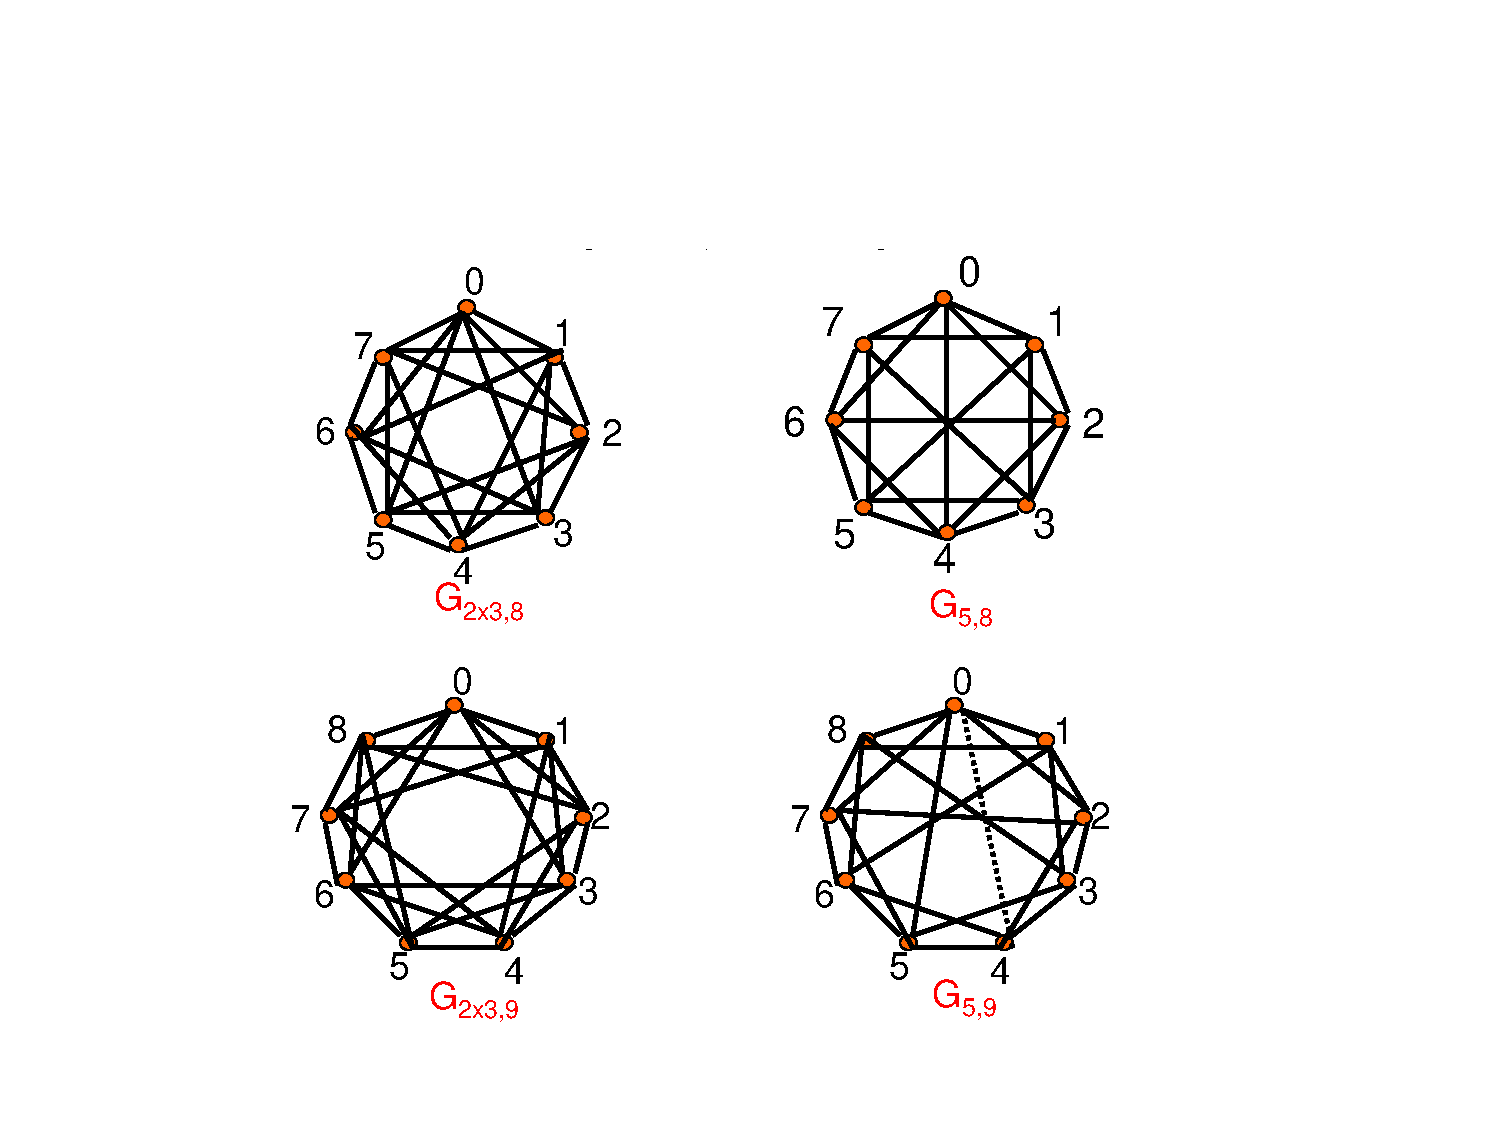
\includegraphics[width = 0.9\linewidth]{maxbian.pdf}
	 	 \caption{由哈拉里的方法构造的一些图\[G_{k,n}\]}
	 	\end{figure}
	\end{enumerate}
\end{document}
